\section{Methodology}

TopoBDA (Figure \ref{fig: TopoBDA_overview}) starts by extracting Bird’s Eye View (BEV) features from multi-camera 360-degree imagery. A transformer decoder then processes these BEV features within its cross-attention mechanism using a sparse query approach. In this approach, each query corresponds to a centerline instance rather than individual points, which improves computational efficiency. Subsequently, the decoder predicts Bezier control points for each instance query which are then converted into dense polyline points via matrix multiplication. The Bezier representation offers a compact and compressed formulation, reducing computational complexity at the regression heads \cite{feng2022rethinking, qiao2023end, li2023graph}. Additionally, each centerline query predicts an instance mask for auxiliary loss, though these masks are not utilized during inference.

\begin{figure}[tb]
  \centering
  \includegraphics[width=\linewidth]{TopoBDA.pdf}
  \caption{Overview of the TopoBDA architecture. The TopoBDA architecture is based on the instance query concept. The extracted BEV features from the multiple camera images are fed into the transformer decoder. The decoder outputs Bezier control points for each query, which are then converted into centerline instances via matrix multiplication. Additionally, each centerline query predicts instance masks, but only during training.}
  \label{fig: TopoBDA_overview}
\end{figure}


In the TopoBDA architecture, the BEV feature extraction  (Figure \ref{fig: TopoBDA_overview}) starts with a set of $N$ images, $\{\mathbf{I}_{i}\}_{i=1}^N$, each having a dimension of $H_I \times W_I \times 3$, with $H_I$ and $W_I$ representing the height and width, respectively. These images are first converted into perspective view features, $\{\mathbf{F}_{PV_i}\}_{i=1}^N$, using a feature extraction function $f_{PV}$, such that $\mathbf{F}_{PV_i} = f_{PV}(\mathbf{I}_i)$ and $\mathbf{F}_{PV_i} \in \mathbb{R}^{H_{PV} \times W_{PV} \times C_{PV}}$. These perspective view features are then aggregated and projected into a single Bird's Eye View (BEV) feature map, $\mathbf{F}_{BEV}$, using a projection function $f_{BEV}$. This function can be implemented via Lift-Splat-Shoot (LSS) \cite{philion2020lift, huang2021bevdet, li2023bevdepth}, transformers \cite{li2022bevformer, chen2022efficient, zhou2022cross, wang2023exploring}, or other projection techniques \cite{li2024fast, xie2022m, harley2023simple}. This projection is defined as $\mathbf{F}_{BEV} = f_{BEV}(\{\mathbf{F}_{PV_i}\}_{i=1}^N)$, where $\mathbf{F}_{BEV} \in \mathbb{R}^{H_{BEV} \times W_{BEV} \times C_{BEV}}$. This methodology effectively captures and transforms spatial features into the BEV space, facilitating further analysis and processing within the TopoBDA framework.

Next, the extracted BEV features $\mathbf{F}_{BEV}$ are fed into the transformer decoder, where they are used as the value input in the cross-attention mechanism. Each query, corresponding to a single centerline instance, interacts with $\mathbf{F}_{BEV}$, and Bezier control points are predicted at each decoder layer. The attention mechanism in TopoBDA is based on Bezier Deformable Attention (BDA) and it is guided by these predicted Bezier control points. Further details of this mechanism are provided in Section \ref{sec: towards_bezier_deformable_attention} and the overall structure of the TopoBDA transformer decoder is provided in Section \ref{sec: BDA_based_transformer_decoder}. 

In the transformer decoder of the TopoBDA, an auxiliary instance mask formulation is also employed (Figure \ref{fig: TopoBDA_overview}). In this formulation, each centerline query predicts not only Bezier control points but also a mask probability map for each instance. This indirect utilization enhances the performance of centerline predictions generated from the Bezier control points. Additionally, replacing the pure L1 matcher with a Mask-L1 mix matcher in the Hungarian matcher process further improves accuracy. The details of the instance mask formulation are provided in Section \ref{sec: indirect_benefits_of_instance_mask_formulation}. This section also introduces the multi-modal data fusion strategy (Section \ref{sec: fusion_methodology}) and the auxiliary one-to-many set prediction loss strategy (Section \ref{sec: one_to_many_set_prediction_loss_strategy}), both of which are integral to the TopoBDA study.



\subsection{Towards Bezier Deformable Attention}
\label{sec: towards_bezier_deformable_attention}

This section explains the transition from Single-Point Deformable Attention (SPDA) to Multi-Point Deformable Attention (MPDA) for methodologies based on Bezier keypoint regression (or Bezier control point regression). This transition replaces traditional deformable attention heads with dense polyline points obtained via matrix multiplication on Bezier control points (Figure \ref{fig: spda_vs_mpda} and \ref{fig: msda_vs_bda}a). 

Next, the concept of Bezier Deformable Attention (BDA) is introduced. BDA enhances the deformable attention mechanism by using Bezier control points. In this approach, traditional attention heads are substituted with the control points of a polyline curve, facilitating more flexible and adaptive attention (Figure \ref{fig: spda_vs_mpda}). In each layer, the predicted control points are utilized to guide the Bezier Deformable Attention process (Figure \ref{fig: msda_vs_bda}b).

\subsubsection{Bezier Curve Representation}

A Bezier curve is a parametric curve frequently used in computer graphics. It is defined by a set of control points, and the curve is a linear combination of these points weighted by Bernstein polynomials.

\sloppy
A Bezier curve \( \mathbf{S}(t) \) of order \( N \) is defined by \( N+1 \) control points $\mathbf{C} = \{\mathbf{c}_0, \mathbf{c}_1, \ldots, \mathbf{c}_N\}$, as shown in Eq. (\ref{eq: parametric_curve_from_bernstein}), where \( B_{n,N}(t) \) are the Bernstein basis polynomials of degree \( N \) which are obtained as in Eq. (\ref{eq: bernsein_parameters}). 

\begin{equation}
\mathbf{S}(t) = \sum_{n=0}^{N} B_{n,N}(t) \mathbf{c}_n, \quad 0 \leq t \leq 1.
\label{eq: parametric_curve_from_bernstein}
\end{equation}

\begin{equation}
B_{n,N}(t) = \binom{N}{n} t^n (1 - t)^{N-n}.
\label{eq: bernsein_parameters}
\end{equation}

The control points \( \mathbf{c}_n \) determine the shape of the Bezier curve, and the Bernstein polynomials \( B_{n, N}(t) \) provide a smooth interpolation between these points.


\subsubsection{Deformable Attention Mechanism}

The deformable attention mechanism enhances traditional attention by adaptively sampling reference points with learned offsets, enabling greater flexibility. Single Point Deformable Attention (SPDA) mechanism is defined as in Eq. (\ref{Eq: SPDA}).
\begin{equation}
\text{SPDA}(\mathbf{q}, \mathbf{V}, \mathbf{p}) = \sum_{m=1}^{M} \sum_{k=1}^{K} A_{m,k} \mathbf{W}_m \mathbf{V}(\mathbf{p} + \Delta \mathbf{p}_{m,k}),
\label{Eq: SPDA}
\end{equation}
where \( \mathbf{q} \) is the query, \( \mathbf{V} \) is the value matrix, \( A_{m,k} \) are the attention weights, \( \mathbf{W}_m \) are learnable weight matrices, \( \mathbf{p} \) is the reference point, \( \Delta \mathbf{p}_{m,k} \) are the offsets, \( M \) is the number of attention heads, \( K \) is the number of sampling points per attention head. In this mechanism, the query \( \mathbf{q} \) attends to the value matrix \( \mathbf{V} \) at positions determined by the reference point \( \mathbf{p} \) and the learned offsets \( \Delta \mathbf{p}_{m,k} \).

\subsubsection{Adaptation of Bezier Regression Methods to Multi-Point Deformable Attention (MPDA)}

\begin{figure}[tb]
  \centering
  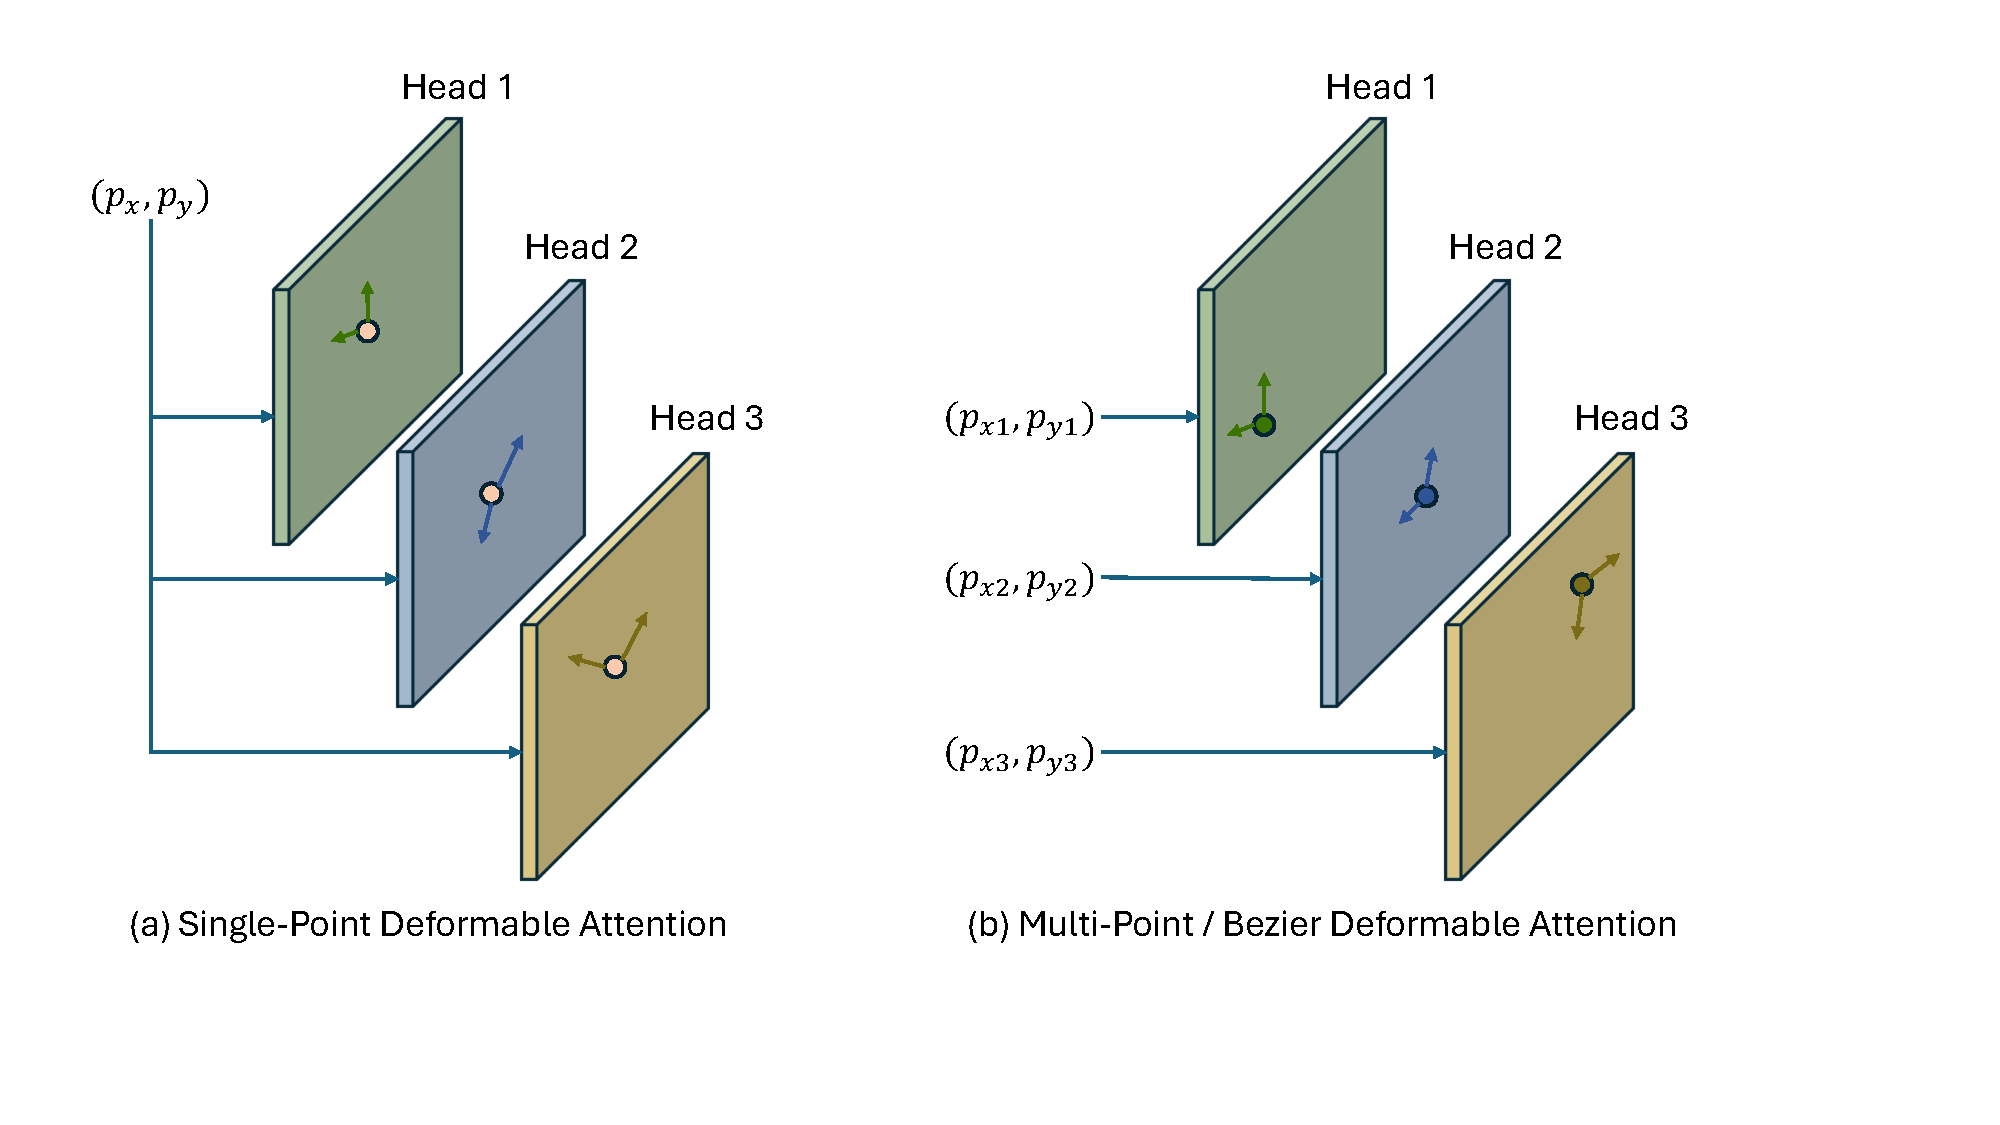
\includegraphics[width=0.7\linewidth]{spda_vs_mpda.pdf}
  \caption{Comparison of Single-Point Deformable Attention (SPDA) with Multi-Point (MPDA) and Bezier (BDA) Deformable Attention. MPDA and BDA share the same underlying mechanism but differ in the selection of multiple reference points $(p_x,p_y)$.}
  \label{fig: spda_vs_mpda}
\end{figure}

This methodology involves extracting \( L+1 \) polyline points $\mathbf{P} = \{\mathbf{p}_0, \mathbf{p}_1, \ldots, \mathbf{p}_L\}$ from the control points $\mathbf{C} = \{\mathbf{c}_0, \mathbf{c}_1, \ldots, \mathbf{c}_N\}$ through Bezier extraction process. These polyline points are then utilized in the deformable attention mechanism. This approach replaces the traditional multi-head attention mechanism, which operates on a single reference point, with a more flexible and adaptive mechanism. Instead of using multiple heads \( M \) on a single point \( \mathbf{p} \), this method employs a single head for each of the dense polyline points \( \mathbf{p}_l \) as shown in Figure \ref{fig: spda_vs_mpda}. By utilizing multiple points distributed along the polyline, this technique captures the thin, elongated characteristics of polylines, thereby enhancing the attention mechanism's ability to model complex patterns and dependencies.

The Multi-Point Deformable Attention (MPDA) mechanism is defined as:
\begin{equation}
\text{MPDA}(\mathbf{q}, \mathbf{V}, \mathbf{P}) = \sum_{l=0}^{L} \sum_{k=1}^{K} A_{l,k} \mathbf{W}_l \mathbf{V}(\mathbf{p}_l + \Delta \mathbf{p}_{l,k}),
\end{equation}
where \( L+1 \) is the number of polyline points, \( K \) is the number of sampling points for each polyline point, \( \mathbf{p}_l \) represents the polyline points extracted from the Bezier control points and members of \( \mathbf{P} \) such that $\mathbf{P} = \{\mathbf{p}_0, \mathbf{p}_1, \ldots, \mathbf{p}_L\}$. 

The polyline points \( \mathbf{p}_l \) can be extracted from the control points using the following formula, which is derived from Eq. (\ref{eq: parametric_curve_from_bernstein}) and Eq. (\ref{eq: bernsein_parameters}):
\begin{equation}
\mathbf{p}_l = \sum_{n=0}^{N} \binom{N}{n} t_l^n (1 - t_l)^{N-n} \mathbf{c}_n,
\label{eq: formula_polyline_points}
\end{equation}
for \( l = 0, 1, \ldots, L \), where \( t_l \) are uniformly spaced within the interval \([0, 1]\). Eq. (\ref{eq: formula_polyline_points}) demonstrates that adapting MPDA to the Bezier keypoint concept necessitates converting Bezier control points into polyline points. This conversion is implemented through matrix multiplication in each decoder layer, as illustrated in Figure \ref{fig: msda_vs_bda}a. The detailed process of this implementation is provided in Supplementary Section~\ref{sup_sec: mf_from_bez_to_poly} of the supplementary materials.

\begin{figure}[tb]
  \centering
  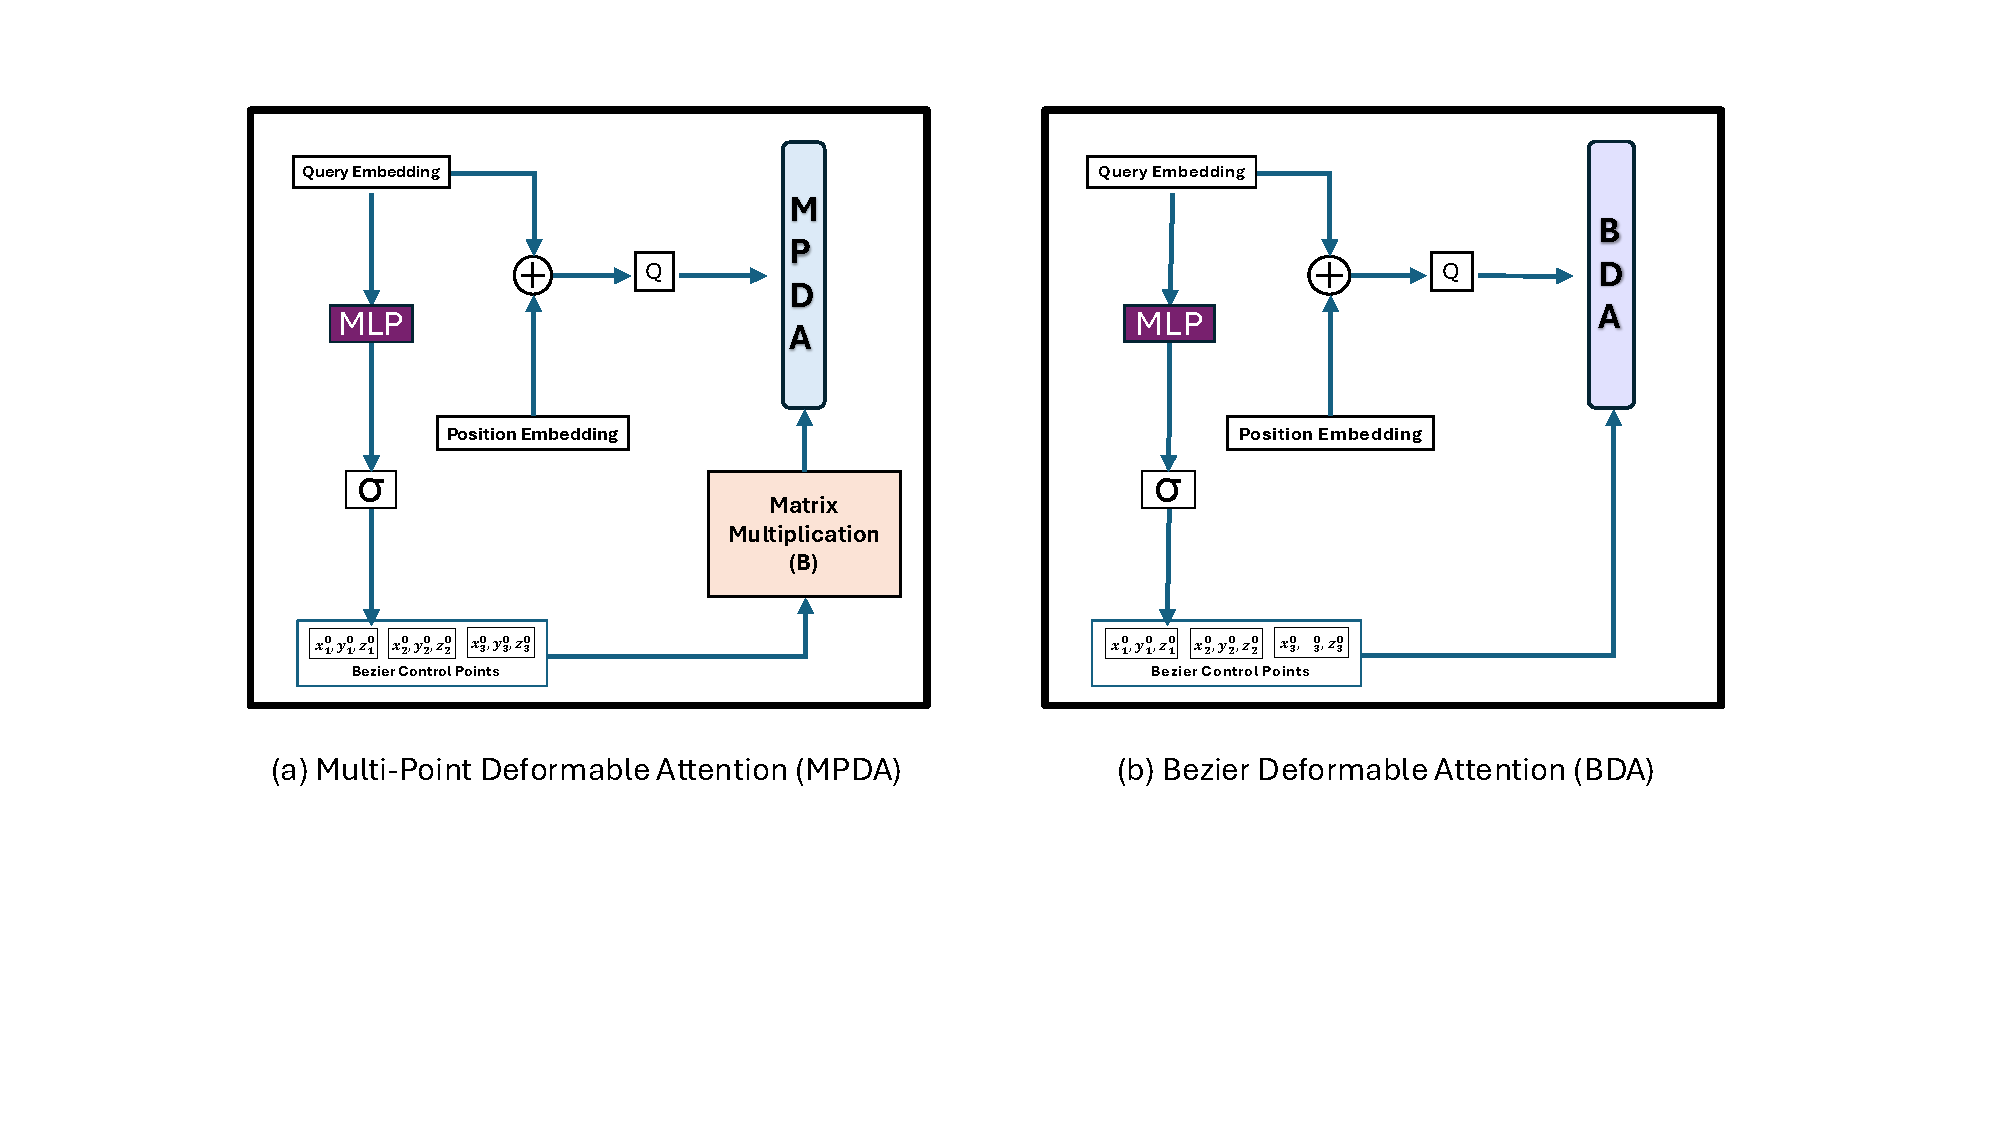
\includegraphics[width=0.8\linewidth]{msda_vs_bda.pdf}
  \caption{Comparison of Multi-Point Deformable Attention (MPDA) and Bezier Deformable Attention (BDA): MPDA necessitates an additional matrix multiplication block within each transformer decoder. Despite their different input utilizations as reference points, the mechanisms of MPDA and BDA blocks are fundamentally the same.}
  \label{fig: msda_vs_bda}
\end{figure}

\subsubsection{Bezier Deformable Attention}

BDA enhances the traditional multi-head attention mechanism by replacing the single-point focus \( \mathbf{p} \) with control points \( \mathbf{c}_n \) of the Bezier curve. From this perspective, the inherent mechanism of BDA is the same with MPDA as shown in Figure \ref{fig: spda_vs_mpda}. Unlike MPDA, which relies on dense polyline points, BDA directly uses these control points as reference points within the deformable attention mechanism. This approach eliminates the need for converting control points to polyline points in each decoder layer (Figure \ref{fig: msda_vs_bda}), reducing computational complexity slightly. By predicting Bezier control points and focusing attention around them, BDA improves the learning process, leading to more effective and accurate predictions. From a theoretical computational complexity standpoint, there is no difference between the attention mechanism of SPDA and BDA, as the only modification lies in the reference points that guide attention across different heads. However, SPDA requires learning an additional reference point learning mechanism in polyline detection structures, which increases the complexity slightly.  


The Bezier Deformable Attention (BDA) mechanism is defined as:
\begin{equation}
\text{BDA}(\mathbf{q}, \mathbf{V}, \mathbf{C} ) = \sum_{n=0}^{N} \sum_{k=1}^{K} A_{n,k} \mathbf{W}_n \mathbf{V}(\mathbf{c}_n + \Delta \mathbf{p}_{n,k}),
\end{equation}
where \( N+1 \) is the number of control points, \( K \) is the number of sampling points for each control point, \( \mathbf{c}_n \) represents the control points and members of $\mathbf{C}$ such that $\mathbf{C} = \{\mathbf{c}_0, \mathbf{c}_1, \ldots, \mathbf{c}_N\}$. In this formulation, each control point \( \mathbf{c}_n \) acts as a head in the attention mechanism, allowing the model to attend to different parts of the input sequence based on the shape of the Bezier curve. This approach provides a more flexible and adaptive attention mechanism that can better capture the spatial structure of polylines.

To summarize, the key distinction between SPDA, MPDA, and BDA lies in how reference points are utilized across attention heads. From a computational complexity perspective, these mechanisms are nearly equivalent when the number of attention heads is the same. However, SPDA introduces slight overhead due to its additional reference point learning, while MPDA incurs cost from converting control points into polyline points. BDA avoids this by directly using Bezier control points.


\subsection{Bezier Deformable Attention Based Transformer Decoder}
\label{sec: BDA_based_transformer_decoder}

\begin{figure}[tb]
  \centering
  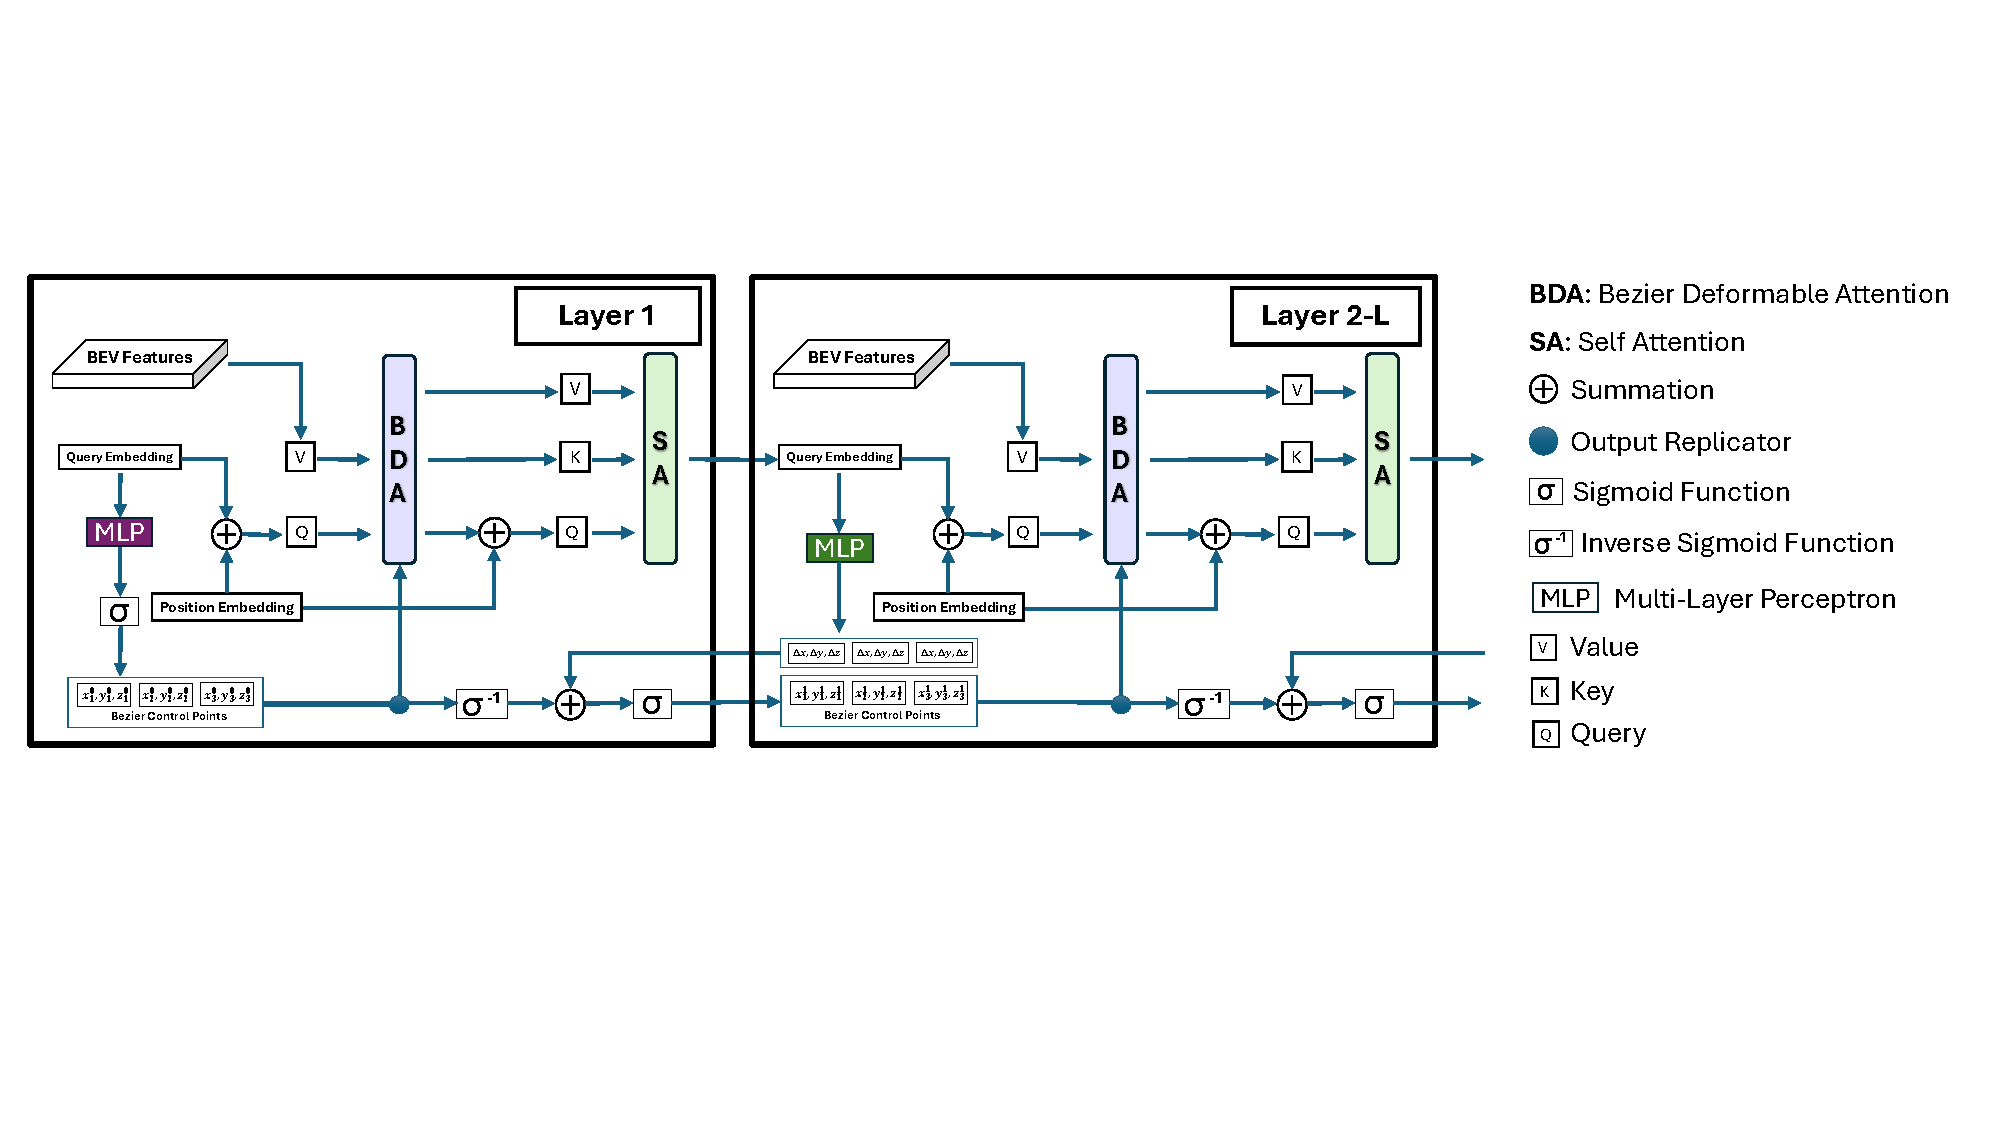
\includegraphics[width=\linewidth]{BDA_layers.pdf}
  \caption{This figure visualizes the layers of TopoBDA, each driven by Bezier Deformable Attention (BDA) using control points predicted through iterative refinement. Note that iterative refinement is not applicable to the first layer, which uses direct prediction.}
  \label{fig: bezier_deformable_attention_detail}
\end{figure}

The overview of the general pipeline of each layer in the transformer decoder of TopoBDA is shown in Figure \ref{fig: bezier_deformable_attention_detail}. The step-wise operation detail of the TopoBDA decoder is also shown in Supplementary Algorithm~\ref{sup_alg: topobda} in Section \ref{sup_sec: algorithm_topobda_decoder}. The iterative refinement-based Bezier control points prediction process involves several steps:

\begin{enumerate}
    \item \textbf{Control Points Generation (First Layer):}
    The control points of each centerline instance are obtained in a normalized format using a Multi-Layer Perceptron (MLP) and a sigmoid function:
    \begin{equation}
        \mathbf{C}_{norm}^{(1)} = \sigma(\text{MLP}_{B}^{(1)}(\mathbf{E}_{query}^{(1)})),
    \end{equation}
    where $\mathbf{C}_{norm}^{(1)} = \{\mathbf{c}_0, \mathbf{c}_1, \ldots, \mathbf{c}_N\}$, and each $\mathbf{c}_i$ consists of normalized (scaled to [0,1]) $x$, $y$, and $z$ coordinates. $\mathbf{E}_{query}^{(1)}$ is the query embedding at the first layer.

    \item \textbf{Bezier Deformable Attention (BDA):}
    The predicted control points are fed into the BDA layer to guide attention. BDA defines the query as the sum of positional embedding and query embedding, while the BEV features serve as the value:
    \begin{equation}
    \begin{aligned}
        \mathbf{Q}_{BDA}^{(l)} = \mathbf{E}_{query}^{(l)} + \mathbf{P}^{(l)}, \\
        \mathbf{A}_{BDA}^{(l)} = \text{BDA}(\mathbf{Q}_{BDA}^{(l)}, \mathbf{F}_{BEV}, \mathbf{C}_{norm}^{(l)}),
    \end{aligned}
    \end{equation}
    where $\mathbf{Q}_{BDA}^{(l)}$ is the combined query embedding and positional embedding at layer $l$, and $\mathbf{A}_{BDA}^{(l)}$ is the output of the BDA layer.

    \item \textbf{Self-Attention:}
    Self-attention follows the output of BDA and utilizes the same positional embedding:
    \begin{equation}
        \mathbf{A}_{SA}^{(l)} = \text{SelfAttention}(\mathbf{A}_{BDA}^{(l)}, \mathbf{P}^{(l)}),
    \end{equation}
    where $\mathbf{A}_{SA}^{(l)}$ is the output of the self-attention layer at layer $l$. The output of the self-attention layer, $\mathbf{A}_{SA}^{(l)}$, serves as the query embedding $\mathbf{E}_{query}^{(l+1)}$ for the next layer.

    \item \textbf{Iterative Process in Subsequent Layers:}
    In subsequent layers, the process repeats, but with MLP layers predicting Bezier control points differences. These differences are summed in the inverse sigmoid domain before being transformed back:
    \begin{equation}
    \begin{aligned}
        \Delta \mathbf{C}^{(l)} = \text{MLP}_{B}^{(l)}(\mathbf{E}_{query}^{(l)}), \\
        \mathbf{C}_{inv\_sigmoid}^{(l)} = \sigma^{-1}(\mathbf{C}_{norm}^{(l-1)}) + \Delta \mathbf{C}^{(l)}, \\
        \mathbf{C}_{norm}^{(l)} = \sigma(\mathbf{C}_{inv\_sigmoid}^{(l)}),
    \end{aligned}
    \end{equation}
    where $\Delta \mathbf{C}^{(l)}$ represents the predicted Bezier control points differences at layer $l$, $\mathbf{C}_{inv\_sigmoid}^{(l)}$ is the sum in the inverse sigmoid domain, and $\mathbf{C}_{norm}^{(l)}$ are the updated control points.
\end{enumerate}



\subsection{The Indirect Benefits of Instance Mask Formulation}
\label{sec: indirect_benefits_of_instance_mask_formulation}

The TopoBDA architecture is further enhanced by integrating instance mask formulation in two key areas. First, instance mask loss is used as an auxiliary loss. In each transformer decoder layer, instance masks are predicted for each centerline instance. Second, the Mask-L1 mix matcher is introduced in the Hungarian matcher, combining mask and L1 losses to improve the accuracy of predictions by leveraging both mask and L1 bipartite-matching mechanisms.

\subsubsection{Instance Mask Formulation as an Auxiliary Loss}

\begin{figure}[tb]
  \centering
  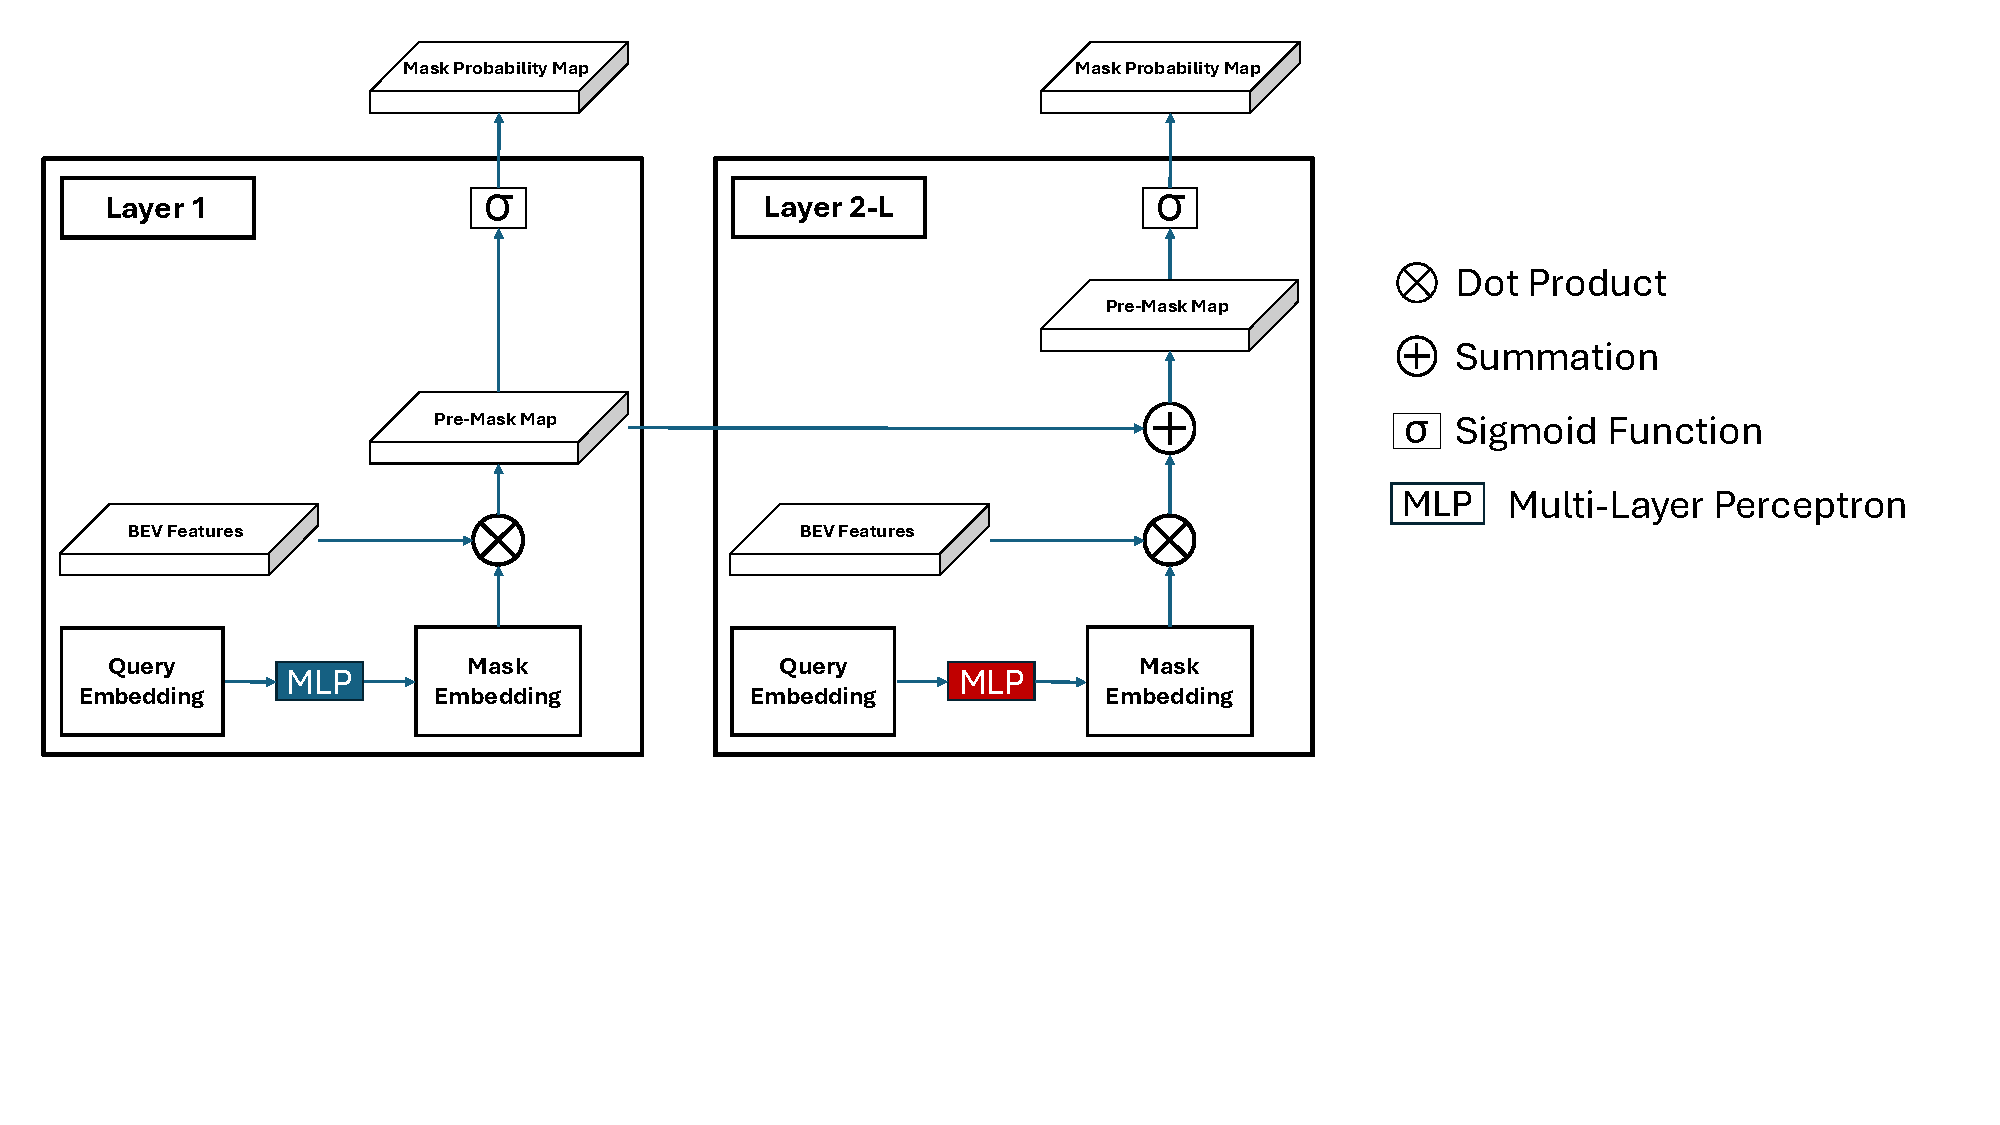
\includegraphics[width=\linewidth]{mask_head.pdf}
  \caption{The implementation of instance mask formulation in the TopoBDA decoder. Query embeddings are converted to mask embeddings by MLP layers. The dot product between BEV features and mask embeddings generates a pre-mask map, which is iteratively summed across layers to produce the final pre-mask map}
  \label{fig: mask_head_in_decoder}
\end{figure}

To achieve this, centerlines are converted into masks using a parameter $W$ in the BEV domain. Utilizing the generated ground truth instance masks, each centerline query in the transformer decoder predicts both Bezier control points and a mask probability map for each centerline instance (Figure \ref{fig: mask_head_in_decoder}). Supplementary Algorithm~\ref{sup_alg: topobda} in Section \ref{sup_sec: algorithm_topobda_decoder} demonstrates the algorithmic details about the mask probability map generation within the TopoBDA transformer decoder. 

The mask probability map generation in the decoder follows several steps:

\begin{enumerate}
    \item \textbf{Mask Embedding Generation:}
    The mask embeddings are generated from the query embeddings using an MLP:
    \begin{equation}
        \mathbf{E}_{mask}^{(l)} = \text{MLP}_{M}^{(l)}(\mathbf{E}_{query}^{(l)}),
    \end{equation}
    where $\mathbf{E}_{mask}^{(l)}$ is the mask embedding at layer $l$ and $\mathbf{E}_{query}^{(l)}$ is the query embedding at layer $l$.

    \item \textbf{Pre-mask Map Generation:}
    A dot product is applied between the BEV features ($\mathbf{F}_{BEV}$) and the mask embedding to generate the pre-mask map:
    \begin{equation}
        \mathbf{P}_{mask}^{(l)} = \mathbf{F}_{BEV} \cdot \mathbf{E}_{mask}^{(l)},
    \end{equation}
    where $\mathbf{P}_{mask}^{(l)}$ is the pre-mask map at layer $l$.

    \item \textbf{Summation of Pre-mask Maps:}
    In consecutive layers, pre-mask maps are summed to refine the mask embeddings at each layer:
    \begin{equation}
        \mathbf{P}_{mask}^{(l)} = \mathbf{P}_{mask}^{(l-1)} + \mathbf{P}_{mask}^{(l)},
    \end{equation}
    where $\mathbf{P}_{mask}^{(l)}$ is the pre-mask map at layer $l$, $\mathbf{P}_{mask}^{(l-1)}$ is the pre-mask map from the previous layer and $\mathbf{P}_{mask}^{(0)}$ is initialized to zero. 

    \item \textbf{Mask Probability Map:}
    The sigmoid function is used to obtain the mask probability maps from the pre-mask maps:
    \begin{equation}
        \mathbf{M}_{prob}^{(l)} = \sigma(\mathbf{P}_{mask}^{(l)}),
    \end{equation}
    where $\mathbf{M}_{prob}^{(l)}$ is the mask probability map at layer $l$ and $\sigma$ is the sigmoid function.
\end{enumerate}


\subsubsection{Mask-L1 Mix Matcher}

The instance mask concept is employed not only in the main loss but also during the bipartite matching (Hungarian matcher). The loss function of the bipartite matching is defined as follows:
\begin{equation}
\mathcal{L}_{\text{l}} = \lambda_{\text{reg}} \mathcal{L}_{\text{reg}} + \lambda_{\text{mask}} \mathcal{L}_{\text{mask}} + \lambda_{\text{cls}} \mathcal{L}_{\text{cls}}.
\end{equation}
When $\lambda_{\text{reg}} = 0$, it operates as a mask matcher, whereas when $\lambda_{\text{mask}} = 0$, it operates as an L1 matcher. When both $\lambda_{\text{reg}}$ and $\lambda_{\text{mask}}$ are non-zero, it is referred to as a Mask-L1 mix matcher. This hybrid matching approach, inspired by the Mask DINO framework \cite{li2023mask}, is adapted to enhance road topology understanding. Experimental results show that utilizing the instance mask formulation in both the main loss and bipartite matching (Hungarian matcher) improves performance. Furthermore, the Mask-L1 mix matcher accelerates the convergence of topology performance.


\subsection{Fusion Methodology}
\label{sec: fusion_methodology}

\begin{figure}[tb]
  \centering
  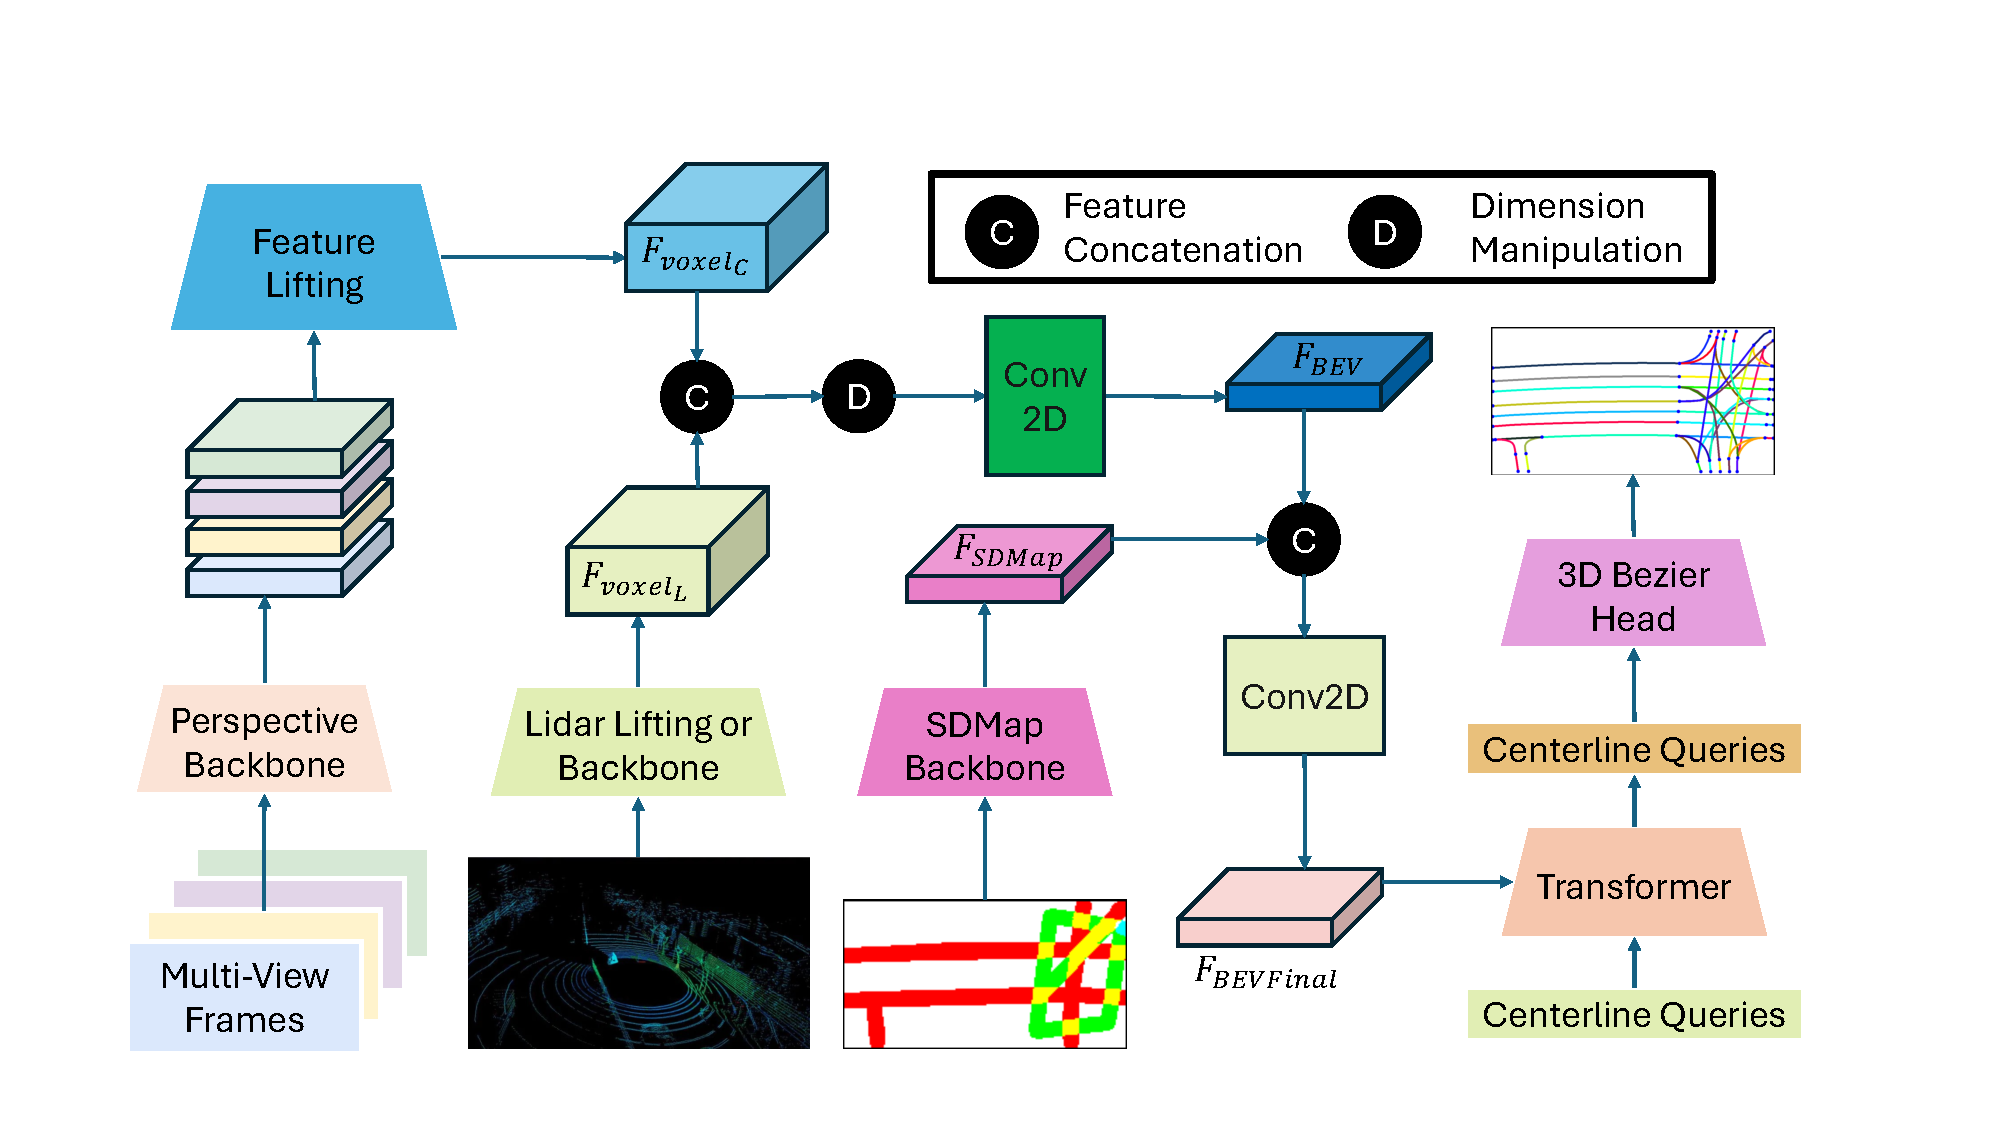
\includegraphics[width=0.9\linewidth]{sensor_fusion.pdf}
  \caption{Sensor fusion pipeline in the TopoBDA architecture.}
  \label{fig: sensor_fusion}
\end{figure}

Sensor fusion for road topology understanding has not been extensively explored in the literature. The sensor and SDMap fusion pipeline used in TopoBDA is illustrated in Figure~\ref{fig: sensor_fusion}. In TopoBDA, camera and lidar features are first concatenated in the voxel space to preserve spatial granularity. This approach differs from BEVFusion studies~\cite{liang2022bevfusion, liu2023bevfusion, tang2023multi}, which typically perform fusion directly in the BEV space. The resulting multi-modal voxel features are merged by flattening the height and channel dimensions, followed by a 2D convolution to obtain BEV features. Although radar features are also fused in the voxel space, they are omitted from Figure~\ref{fig: sensor_fusion} for clarity. SDMap fusion is performed separately in the BEV domain, where SDMap features are concatenated with the BEV features derived from other sensors. The mathematical formulation of the fusion pipeline, including voxelization, multi-modal concatenation, and SDMap integration, is detailed in Supplementary Section~\ref{sup_sec: fusion} of the supplementary materials. 

\subsection{Auxiliary One-to-Many Set Prediction Loss Strategy}
\label{sec: one_to_many_set_prediction_loss_strategy}


To improve training efficiency, an auxiliary one-to-many set prediction loss strategy \cite{jia2023detrs, liao2024maptrv2} is employed. This study, to the best of our knowledge, is the first to perform ablation experiments on this strategy for road topology understanding. Results show that this approach significantly enhances the architecture’s ability to understand road topology.

The auxiliary one-to-many set prediction loss approach involves a smaller decoder and a larger decoder with shared weights. The smaller decoder uses the ground truth set directly, while the larger decoder employs a repeated ground truth set to increase the number of positive samples. During training, both decoders are utilized, while only the smaller decoder is employed during inference. The mathematical background of this loss strategy, including decoder sharing with masking, is provided in Supplementary Section \ref{sup_sec: one_to_many} of the supplementary materials.
